\documentclass{article}

%package imports
\usepackage[dutch]{babel}
\usepackage[backend=biber,style=apa,autocite=inline]{biblatex}
\usepackage{wrapfig}
\usepackage{graphicx}

%meta data
\date{\today}
\title{ITIL Samenvatting}
\author{Wannes De creane, Michiel Schoofs}
\graphicspath{{./imgs/}}


%bib reference
\addbibresource{Bibliografie.bib}

%Custom commando's
\newcommand{\boldit}[1]{\emph{\textbf{#1}}} 
\newcommand{\customref}[1]{\underline{\ref{#1}: \nameref{#1}}}

\begin{document}

	\maketitle
	\section{Inleiding}
	ITIL staat voor Information Technology Infrastructure Library, Dit is een methodiek om aan procesmatig werken te doen binnen in IT. Meerbepaald een praktische “no nonsense approach”, zoals beschreven volgens ITIL®: the basics van \cite{Cater-Steel2006}, voor identificatie, planning, levering en support van IT services voor bedrijven.\\
	
	\par
	\noindent
	ITIL is aldus een leidraad om aan IT Service Management ( ITSM ) te doen, maar wat is dit nu juist? Een service voorziet waarde voor klanten, services die direct door klanten kunnen gebruikt worden noemt men bijgevolg business services een voorbeeld hiervan is bijvoorbeeld “Payroll”, dit is een IT service die gebruikt wordt om informatie bij te houden, compensatie te berekenen en cheques te genereren.\\
	
	\par
	\noindent
	Vaak ziet men de verschillende services van IT en business als een volledig andere wereld. Men gaat dan ook vaak gaan micromanagen en verliest het grote plaatje uit het oog. ITIL suggereert echter een meer holistische en consequente benadering van het ITSM process.\\
	
	\par
	\noindent
	Om de samenhang tussen nieuwe IT services en het bedrijf zonder problemen te laten werken zijn er dus verschillende processen nodig.
	
	\section{Situering van ITIL binnen Business}
	
	\begin{wrapfigure}{L}{0.3\textwidth}
		\centering
		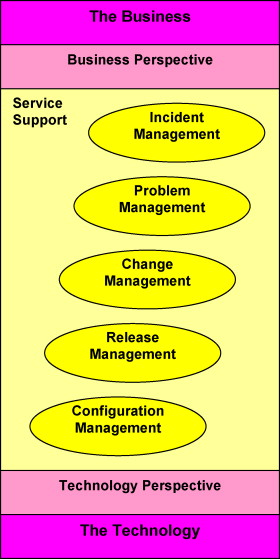
\includegraphics[width=0.25\textwidth]{itil1.jpg}
		\caption{\label{fig1:ItilProcess}This is a figure caption.}
	\end{wrapfigure}
	
	Zoals hierboven reeds kort uitgelegd is ITSM, een collectie van processen en normen voor het beheren,verbeteren en integreren van I.T. services binnen een bedrijf.\\ 
	
	\par
	\noindent
	Historisch gezien, zoals uitgelijnd in de paper van \cite{McNaughton_2010} waren meeste ITSM procedures gepatenteerd en bedrijfsspecifiek. Onder invloed van de ‘Office of Government Commerce’ kwam daar echter verandering in en werd ITIL ontwikkeld dit is een framework van ‘best practices’ om op een succesvolle en consequente manier aan ITSM te doen.\\
	
	\par
	\noindent
	Analoog met de devops beweging is het voornaamste doel om de kloof te dichten tussen I.T. en de bedrijfsvloer. Men ziet I.T. niet als een losstaande eenheid en probeert elke geleverde service op een succesvolle manier te integreren in het bedrijf. Ongeacht van het type (Hardware, software, support,...). De grafiek geeft dan ook een grafische weergave van het ITIL  process.\\
	
	\par
	\noindent
	Zoals aangegeven in Grafiek \ref{fig1:ItilProcess} ziet men opnieuw de twee grote categorieën naar voren komen namelijk de technologie en het bedrijf. Om het nog eens in andere woorden uit te drukken is ITIL de manier om het perspectief van het bedrijf en dat van nieuwe technologie in één lijn te brengen.\\
	
	\noindent
	Hieronder volgen dan ook enkele overzichten van de processen binnen ITIL.
	
	\section{Incident Management Process}
	
	Dit proces staat in voor de levenscyclus van alle incidenten. Het primaire doel is het terugbrengen van de IT service naar de klanten. Dit kan bijvoorbeeld het volledige proces inhouden waar een gebruiker een fout meldt aan de klantenservice, dit wordt doorgegeven naar de IT afdeling en dat op zijn beurt dan onmiddellijk wordt opgelost, zodat de klant snel weer de service kan gebruiken.
	
	\section{Problem Management Process}
	
	Het grootste doel van dit probleem is het voorkomen van een “Incident Management Process” in het geheel, je doet dus aan preventie van incidenten, maar je probeert ook de impact van zo’n incidenten te minimaliseren indien deze niet volledig kunnen vermeden worden. 
	
	\section{Change Management Process}
	
	Dit proces staat voornamelijk in voor het vlot doen verlopen van veranderingen die moeten gebeuren aan de service, in dit proces focust er men dus op dat de service zo goed mogelijk beschikbaar moet blijven terwijl deze veranderingen worden geïmplementeerd. bijvoorbeeld iemand die iets wil veranderen moet deze verandering eerst en vooral melden met alle wijzigingen, deze worden dan wekelijks bekeken door iedereen. Op deze manier probeert men de negatieve impact en consequenties van de wijzigingen op de services te minimaliseren.
	
	\section{Link tussen deze processen}
	Wat is nu juist de link tussen deze verschillende processen? Wel, deze wordt het best geïllustreerd aan de hand van een voorbeeld.\\
	
	\par
	\noindent
	Analoog aan het eerste voorbeeld, waar iemand een probleem meld in de service, en het dan een Incident Management Process doorloopt, gaat men tijdens dit process ook aan Change Management doen, om te zorgen dat potentiële veranderingen geen negatieve impact hebben op de werking van de service.\\
	
	\par
	\noindent
	Eenmaal men aan Incident Management gedaan heeft zou men idealiter ook aan Problem Management moeten doen, dit omdat het niet de bedoeling is dat dit incident nog zal voorkomen. Men doorloopt dus dit process zodat men de volgende keer dit incident niet meer zal tegenkomen, of ervoor kan zorgen dat de impact minder groot is. Ook hier doet men aan Change Management om te zorgen dat eventuele veranderingen geen impact zullen hebben op de service.
	
	\section{Concreet voorbeeld}

	\printbibliography
\end{document}